\documentclass[aspectratio=169]{beamer}
\usetheme{Hannover}

\usepackage{microtype}
\usepackage{amsfonts}
\usepackage{nicefrac}
\usepackage{graphicx}
\usepackage{biblatex}
\usepackage{subcaption}
\usepackage[inkscapepath=svgsubdir]{svg}

\addbibresource{references.bib}

\title{Novelty-Guided Proximal Curriculum Learning}
\author{Jan Malte Töpperwien}
\date{16.09.2024}

\begin{document}
\begin{frame}
  \titlepage
\end{frame}

\section{Introduction}
\begin{frame}
  \begin{columns}[]
    \begin{column}{0.48\textwidth}
      \begin{itemize}
        \item need lots of exploration
        \item sparse rewards -> infrequent learning signal
        \item Use curriculum learning for apprioriate task difficulty -> self-paced
        \item[$\rightarrow$] other approaches often not self-paced and imitation-based
        \item How to set this task difficulty?
      \end{itemize}
    \end{column}
    \hfill
    \begin{column}{0.48\textwidth}
      \begin{figure}
        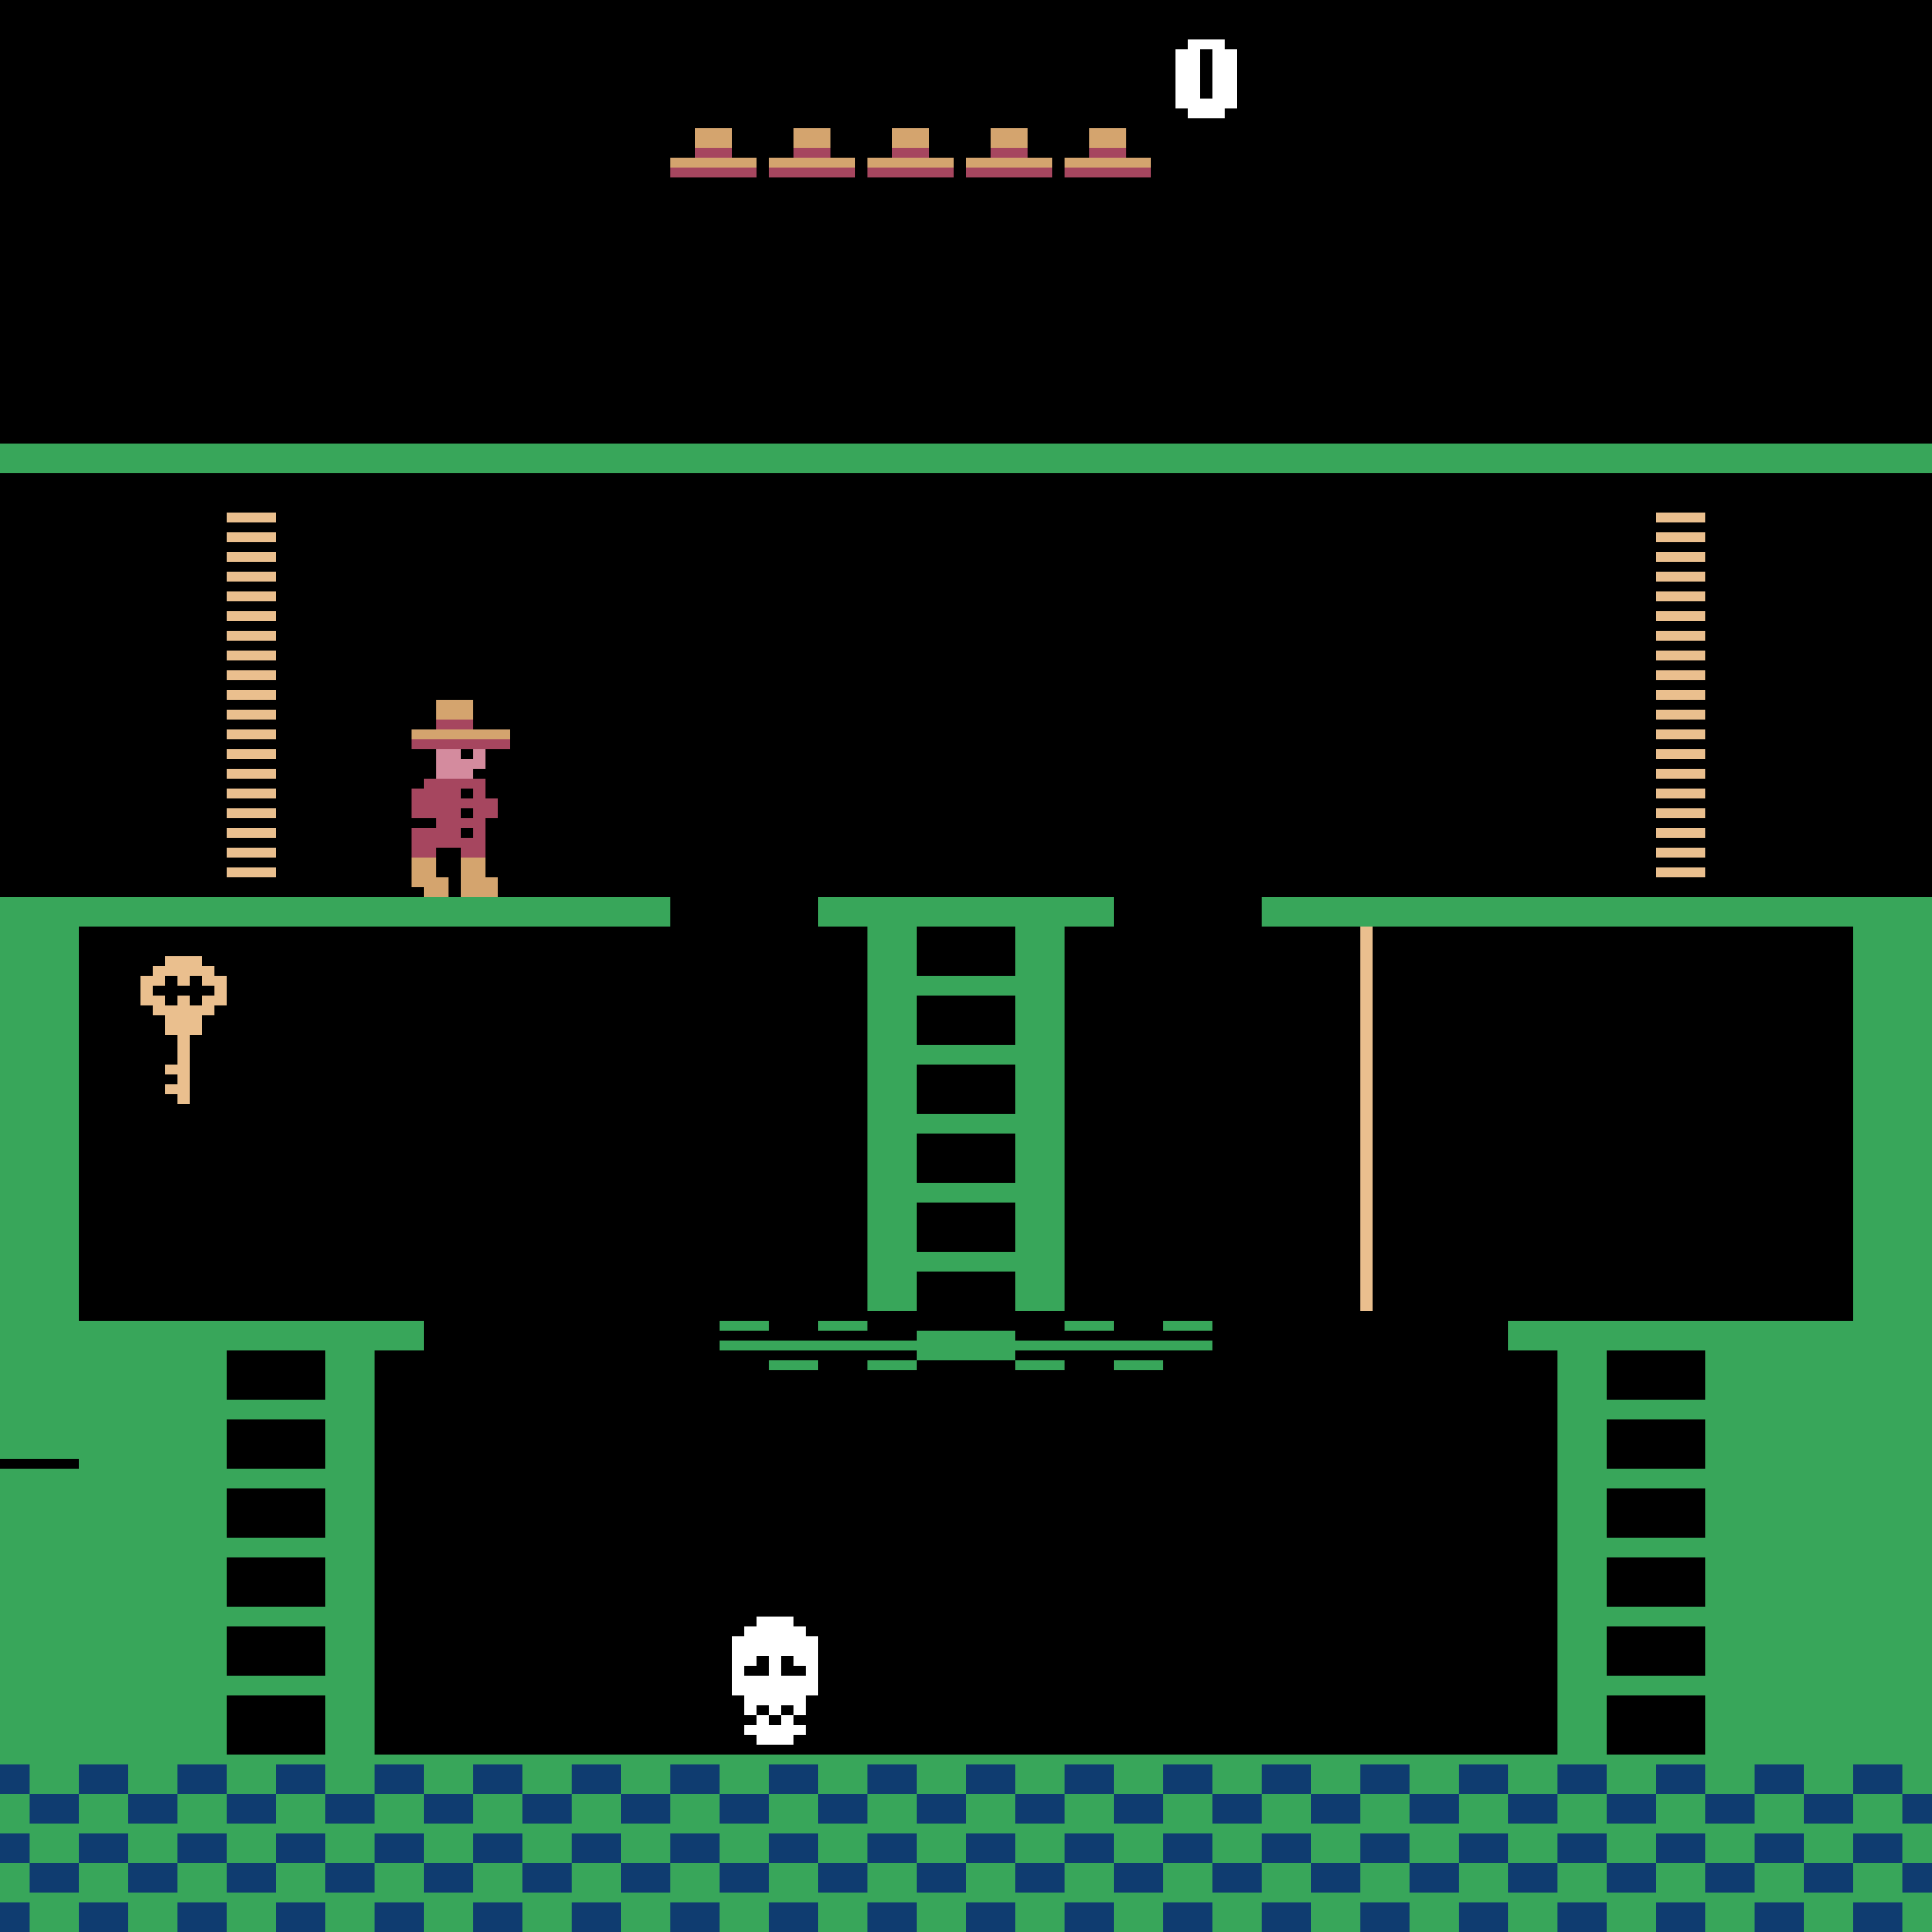
\includegraphics[width=\textwidth, height=\textheight, keepaspectratio]{./images/learning-montezumas-revenge-from-a-single-demonstration}
        % TODO: caption with source
      \end{figure}
    \end{column}
  \end{columns}
\end{frame}

\section{Method}
\begin{frame}{Proximal Curriculum Learning (PCL)~\cite{prox_curr}}
  \begin{itemize}
    \item Set starting states based on \textit{probability of success} $PoS$
    \item $PoS = 0.5 \rightarrow$ avoid tasks the agent fails on and avoid already learnt tasks
    \item Approximate $PoS$ for a given state by using the agents value function $V$
    \item $PoS$ is scaled to $[0, 1]$
    \item distribution over pool of states $S_{init}$ where $PoS = 0.5$ is preferred
  \end{itemize}
  \vfill
  \pause
  Problems:
  \begin{itemize}
    \item $V$ initialized randomly
    \item $V$ inaccurate for seldomly seen states
    \item states may get $PoS$ of 0 or 1 and never get chosen
  \end{itemize}
\end{frame}

\begin{frame}{State Novelty}
  Exploration may help us fix the problem.
  \begin{itemize}
    \item novelty state $\sim$ V inaccuracy
    \item[$\rightarrow$] explore seldomly seen states
    \item set starting state based on state novelty
  \end{itemize}
\end{frame}

\begin{frame}{Novelty-Guided Proximal Curriculum Learning NGPCL}
  \begin{itemize}
    \item incorporate novelty by creating distribution over $S_{init}$
    \item[$\rightarrow$] faster $V$ convergence
    \item[$\rightarrow$] skip environment steps needed for intrinsic reward
    \item overlay both distributions by using weighted sum
  \end{itemize}
\end{frame}


\section{Results}
\begin{frame}{Environments}
  \begin{figure}
    \begin{subfigure}{0.48\textwidth}
      \centering
      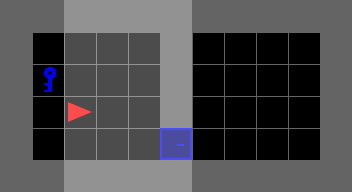
\includegraphics[width=\textwidth, height=\textheight, keepaspectratio]{./images/unlock-v0.png}
      \caption{Unlock}
    \end{subfigure}
    \begin{subfigure}{0.48\textwidth}
      \centering
      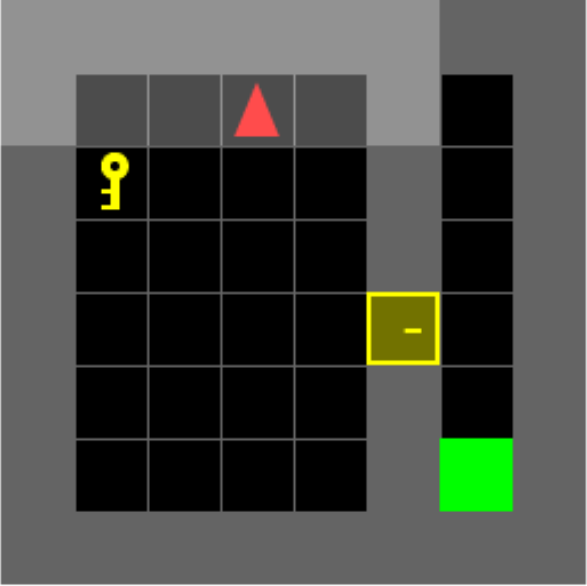
\includegraphics[width=0.75\textwidth, height=\textheight, keepaspectratio]{./images/doorkey-8x8-v0.png}
      \caption{DoorKey-8x8}
    \end{subfigure}
    \caption{Environments used for experiments~\cite{minigrid}. Key was added to observation.}
  \end{figure}
\end{frame}

\begin{frame}{Setup}
  \begin{itemize}
    \item $S_{init}$ over all states, not evolving
    \item Random Network Distillation (RND)~\cite{rnd} as state novelty implementation
    \item Hyperparameters and architectures optimized by bayesian optimization using SMAC~\cite{smac}
  \end{itemize}
\end{frame}

\begin{frame}
  \begin{figure}
    \begin{subfigure}{0.48\textwidth}
      \centering
      \includesvg[width=\textwidth]{../plots/unlock/results_per_approach_paper.svg}
      \caption{Unlock}
    \end{subfigure}
    \begin{subfigure}{0.48\textwidth}
      \centering
      \includesvg[width=\textwidth]{../plots/doorkey8/results_per_approach_paper.svg}
      \caption{Doorkey-8x8}
    \end{subfigure}
    \caption{Rewards over training steps starting from usual starting state (NGPCL). 5 seeds with 95\% CI.}
  \end{figure}
\end{frame}

\begin{frame}
  \begin{figure}
    \begin{subfigure}{0.48\textwidth}
      \centering
      \includesvg[width=\textwidth]{../plots/unlock/results_combined_paper.svg}
      \caption{Unlock}
    \end{subfigure}
    \begin{subfigure}{0.48\textwidth}
      \centering
      \includesvg[width=\textwidth]{../plots/doorkey8/results_combined_paper.svg}
      \caption{Doorkey-8x8}
    \end{subfigure}
    \caption{Rewards over the training steps given seed (NGPCL).}
  \end{figure}
\end{frame}

\section{Discussion}
\begin{frame}
  Results:
  \begin{itemize}
    \item some seeds showed fast learning
    \item ... others failed to solve the environment
  \end{itemize}
  \vfill
  \begin{columns}[T]
    \begin{column}{0.48\textwidth}
      Things to try:
      \begin{itemize}
        \item schedule for overlay parameter of distributions
        \item interleave PCL with RND
        \item try other state novelty approaches
        \item (dynamic) $S_{init}$ determination
      \end{itemize}
    \end{column}
    \begin{column}{0.48\textwidth}
      Environments to evaluate:
      \begin{itemize}
        \item dense rewards
        \item big/continuous state- and/or action-spaces
        \item reward space being not convex
      \end{itemize}
    \end{column}
  \end{columns}
\end{frame}

\end{document}
